\chapter{Problem statement and solving methodology}
\label{ch4}
This chapter describes the elements and methodology used to solve the forecasting and control problems.

\section{Problem statement}
\label{sec:4ps}
This thesis focuses on \gsl{ANM} and the problem faced by a \gsl{DSO} to maintain the network within its operational limits. In particular, the system operator evaluates whether at a given moment there will be a voltage problem. In this way, the \gls{DSO} can proceed with some actions, like applying curtailment to generator devices or control their reactive power, to maintain the voltage inside a safe range.\\

For this problem, we assume that the \gls{DSO} knows the following information:
\begin{itemize}
    \item The network topology: the number of buses, loads and generators, the lines' length, the distance between the connected buses, and the distance between each load and generator from the bus they are connected to. Moreover, the impedance of the lines is known.
    
    \item The active and reactive power of some loads at each time step. \\
    In a real case it would be possible that some values may not available mainly for two reasons: \emph{a)} for that particular load there are no measurements at all for the lack of sensors or for privacy reasons; or \emph{b)} communication problem, so the sensor recording was lost. These cases are not considered in this thesis, so all the information is available.
    
    \item The type of \gsl{DER} device connected to each bus. If the \gls{DER} device is directly connected to the medium voltage grid, the active power and reactive power are considered known. 
\end{itemize}

This data is used to calculate the power flow of the network and obtain more information like the voltage magnitude at each bus, lines' loading and other values. This calculation can be performed with any power system analysis tool, like for example Pandapower.\\

% Moreover, since the power flow depends on the power injection of the different elements, it is possible to create some possible cases changing the active and reactive power of the devices. These cases can be generated multiplying the time series by some scaling factors to increase or decrease the injection values.  \\

A power network can be represented as a direct graph $\mathsf{G}(\mathcal{N},\mathcal{E})$, where \gls{N} is a set of nodes, also called buses ($\mathcal{B}$), in the network; \gls{E} $\subseteq \mathcal{N} \times \mathcal{N}$ is the set of directed edges linking two buses together, also called lines. The notation \gls{e} $\in \mathcal{E}$ refers to the directed edge with sending bus $i$ and receiving bus $j$. Each bus might be connected to several devices, which may inject or withdraw power from the grid. The set of all devices is denoted by \gls{D} that can be either loads \gls{L} or generators \gls{G}. Let's also define \gls{T} as the set of transformers. \\

% https://arxiv.org/ftp/arxiv/papers/2102/2102.05657.pdf
The \gls{DSO} considers the behaviour of the network over a set of discrete time steps $t \in \{1,2,...,T-1,T\}$ of length $\Delta t$, with, $T \in \mathbb{N}$, the last time step of the time series’ horizon. A time step is considered as a snapshot of the system at one particular point in time. \\ 

The \gls{DSO} can have access to some information, let's define $\textbf{I}$ as the information domain. This information can be divided in static information like the network topology, and the observation $\mathbf{O_t}$ collected at every time step $t$ like the loads and generators' active and reactive power and the buses' voltage magnitude and lines' loading. The information at time step $I_t$ can be defined as:
\begin{align*}
    \mathbf{I_t} & \in \mathbf{I}, \text{with} \, t \in \{1,2,...,T-1,T\} \\
    \mathbf{I_t} & = [\mathbf{{static}} \, \mathbf{{information}}, \mathbf{O_t}]
\end{align*}
\noindent In general power networks are not static, since the operators can modify their topology, for example changing the connections due to some incidents on the lines. In this thesis, the network topology is considered as static, so that no changes are applied on the network during the whole time series' horizon.\\

\noindent An instance of the observation $\mathbf{O_t}$ can be:
\begin{equation*}
    \mathbf{O_t} =  [
            \mathbf{\mathcal{L}^p_{t}}, 
            \mathbf{\mathcal{L}^q_{t}}, 
            \mathbf{\mathcal{G}^p_{t}},
            \dots ]
\end{equation*}
\noindent where $\mathbf{\mathcal{L}^p_{t}}$ and $\mathbf{\mathcal{L}^q_{t}}$ are active and reactive power of loads $\mathcal{L}$ at timestamp $t$; $\mathbf{\mathcal{G}^p_{t}}$ is the active power of the generators $\mathcal{G}$ at time $t$; some other variables can be included in the observation $\mathbf{O_t}$ for example the buses' voltage magnitudes or the loading percentage of each line, etc.\\

For the forecasting part, the operator predicts if the system, at some given $t+n$ future time steps, will be in a critical condition. As mentioned in \ref{sec:3tss}, the network is considered in a critical condition if any of its elements is in an unsafe situation, for example an over voltage condition. Let define $\textbf{C}$ as the list of critical situations and $C_t$ the critical situation at time step $t$, with $C_t \in \{0,1\}$.  \\
For predicting whether the system will be in a critical situation or not, the \gls{DSO} considers the history of the system only for $h$ preceding steps, with $h \in \mathbb{N}^+$. \\

% Let also define the function $f_\mathcal{N}$ that given the information from a particular network can elaborate this information and output some values, that represent the forecasting of a critical situation. \\
% It is possible to summarize all the information under the relationship:
% \begin{equation} \label{eq:fmapping}
%     %C = f_\mathcal{N}(I_{t-h+1},I_{t-h+2},\dots,I_{t-1},I_{t})
%     \hat{\textbf{C}} = f_\mathcal{N}(\textbf{I})
% \end{equation}
% \noindent where $\hat{\textbf{C}}$ represents the forecasted values of the system given the information $\textbf{I}$. A single instance $\hat{C}_{t+i}$ ($\hat{C}_{t+i} \in \{0,1\}$) states if the system is critical ($\hat{C}_{t+i}=1$) or not ($\hat{C}_{t+i}=0$), with $i \in \{1,2,\dots,n-1,n\}$ and $n \in \mathbb{N}^+$. \\

% For the control part, an agent is trained to solve the voltage problems. Its goal is to choose some actions adjusting active and reactive power of the generators that maximise a reward function given some network information as input.

\section{Solving methodology}
\label{sec:4sm}
\subsection{Forecasting}
The goal of this section regards the explanation of the solving methodology for aim \ref{aim2}, that is, to train a classifier that can forecast whether in the future there will be some over voltage problems.\\

As a supervised task, the time series are separated in training and testing dataset; in particular, the data is divided in windows of length, $h$ for the inputs $\textbf{x}$ and length $n$ for the outputs $\textbf{y}$. \\

There are many ways and combinations of how to choose the information used for the input $\textbf{x}$s. In this thesis, three combinations are tested:

\begin{enumerate}[label=\textbf{\roman*)}]
    \item \label{onlyV} Considering only the voltage information at each bus.
    \begin{equation}
      \begin{aligned}
        \textbf{x}  &= [\mathbf{\mathcal{B}^{V}_{t-h+1}}, \mathbf{\mathcal{B}^{V}_{t-h+2}}, \dots, \mathbf{\mathcal{B}^{V}_{t-1}}, \mathbf{\mathcal{B}^{V}_{t}}]
      \end{aligned}
    \end{equation}
    \noindent where $\mathbf{\mathcal{B}^{V}_{t}}$ is the voltage level \gls{V} of every bus $\mathcal{B}$ at timestamp $t$. It can be represented as a matrix, as follows:
    \begin{equation*}
      \begin{aligned}
        \textbf{x}  &= 
        \begin{bmatrix}
        \mathcal{B}^{V}_{t-h+1,1} & \mathcal{B}^{V}_{t-h+2,1} & \cdots & \mathcal{B}^{V}_{t-1,1} & \mathcal{B}^{V}_{t,1} \\
        & & & & \\
        
        \mathcal{B}^{V}_{t-h+1,2} & \mathcal{B}^{V}_{t-h+2,2} & \cdots & \mathcal{B}^{V}_{t-1,2} & \mathcal{B}^{V}_{t,2} \\
        & & & & \\
        
        \vdots & \vdots & \ddots & \vdots & \vdots \\
        & & & & \\
        
        \mathcal{B}^{V}_{t-h+1,|\mathcal{B}|-1} & \mathcal{B}^{V}_{t-h+2,|\mathcal{B}|-1} & \cdots & \mathcal{B}^{V}_{t-1,|\mathcal{B}|-1} & \mathcal{B}^{V}_{t,|\mathcal{B}|-1} \\
        & & & & \\
        
        \mathcal{B}^{V}_{t-h+1,|\mathcal{B}|} & \mathcal{B}^{V}_{t-h+2,|\mathcal{B}|} & \cdots & \mathcal{B}^{V}_{t-1,|\mathcal{B}|} & \mathcal{B}^{V}_{t,|\mathcal{B}|} \\
        \end{bmatrix}
      \end{aligned}
    \end{equation*}
    \noindent where $\mathcal{B}^{V}_{t,i}$ is the voltage level \gls{V} of a single bus $i$ at timestamp $t$. \\
    
    \item \label{LpqandGp} Considering active and reactive power of loads and active power of generators.
    \begin{equation}
      \begin{aligned}
        \textbf{x}  &= [
            \mathbf{\mathcal{L}^p_{t-h+1}}, \mathbf{\mathcal{L}^q_{t-h+1}}, \mathbf{\mathcal{G}^p_{t-h+1}},
            \dots,
            \mathbf{\mathcal{L}^p_{t}}, 
            \mathbf{\mathcal{L}^q_{t}}, 
            \mathbf{\mathcal{G}^p_{t}}]
      \end{aligned}
    \end{equation}
    \noindent where $\mathbf{\mathcal{L}^p_{t}}$ and $\mathbf{\mathcal{L}^q_{t}}$ are, respectively, the active and reactive power of all loads \gls{L} at timestamp $t$ and $\mathbf{\mathcal{G}^p_{t}}$ is the active power of each generator \gls{G} at timestamp $t$. Similarly to the first case \ref{onlyV}, a matrix can be written, but it is omitted.
    
    \item \label{GpandTpq} Considering active power of generators and the active and reactive power at the transformer on the HV/MV substation.
    \begin{equation}
      \begin{aligned}
        \textbf{x}  &= [
            \mathbf{\mathcal{G}^p_{t-h+1}}
            \mathcal{T}^p_{t-h+1},
            \mathcal{T}^q_{t-h+1}, 
            \dots,
            \mathbf{\mathcal{G}^p_{t}}, 
            \mathcal{T}^p_{t}, 
            \mathcal{T}^q_{t}]
      \end{aligned}
    \end{equation}
    \noindent where $\mathcal{T}^p_{t}$ and $\mathcal{T}^q_{t}$ are, respectively, the active and reactive power of the transformer at timestamp $t$.
    
    \item \label{case4} Since the considered dataset is unbalanced, some techniques usually used when dealing with these kinds of datasets are employed. The techniques are, as mentioned in \ref{ssec:unbalan}, over and under sampling and set weights for each class.\\
    These techniques are tested on the best and worst performing models of all the aforementioned combinations.
    % \ref{onlyV}, \ref{LpqandGp}, \ref{GpandTpq}
\end{enumerate}
\noindent Different combinations are considered because it is interesting to check how the model performs with different kinds of data; moreover, the information a \gls{DSO} can have access to can be limited, so some cases are more realistic than others. In particular, \gls{DSO} usually has access to only a limited amount of data: for small loads (households, ...) the active and reactive powers are not available at every instant (they are only after some period of time, after the bill is issued), in general the more a device is close to the transformer, the more information a \gld{DSO} has access to, so the combination \ref{GpandTpq} would be the most appropriate for a MV network.\\


\noindent For the labels, $\textbf{y}$ can be defined as: 
\begin{equation} \label{eq:labels}
    \begin{aligned}
        \textbf{y} = [C_{t+1},C_{t+2}, \dots, C_{t+n-1},C_{t+n}]
    \end{aligned}
\end{equation}
\noindent where $C_t$ is the condition of the system at timestamp $t$, with $C_t=1$ if the network is in a critical situation or $C_t=0$ if it is in a normal situation and $n$ is the number of future time steps considered, with $n \in \mathbb{N}^+$. \\

For what concerns $h$, the number of history step considered and $n$, the number of future steps to forecast, these are not hyperparameter to be optimised, but are values that depend on the problem and the task that a \gls{DSO} is trying to solve. In particular, choosing a value of $h$ depends on the amount of data the \gls{DSO} can access to, the computation cost and the time to get an answer; while $n$, depends on the kind of forecasting the \gls{DSO} wants to apply, either short planning (from minutes to hours), medium-term planning (from hours to days) or long-term planning (many days). It has also to be noted that it is expected that higher values of $n$ would get less accurate forecasting.\\

The couples $\{\textbf{x},\textbf{y}\}$ are divided in training, validation and test set, with the following ratios: $0.7$, $0.2$, $0.1$.

\begin{figure}[H]
\centering
    
\includegraphics[width=0.9\linewidth]{images/MVOberr/Time Series Windowing.png}
\caption[Time series windowing]{Division of the time series in windows of length $h$ as past information and length $n$ as forecasting values.}
\label{fig:timewindow}
\end{figure}
\noindent Figure \ref{fig:timewindow} shows how the time series are separated in input and output lists: the input $\textbf{x}$ is generated taking the raw information of size $h$ ($\textbf{x}$ is different for each combination used), and the output $\textbf{y}$ is generated taking the information about the buses' voltage magnitudes of length $n$ and converted to a binary value that represent whether the system is in a critical situation or not as mentioned in \ref{sec:3tss} ($\textbf{y}$ is the same for each combination considered). \\

For the forecasting part, only over voltage situations are considered. \\
The followings are the critical states' distribution in training, validation and test sets.
\begin{algorithm}[h]
    \State Number of over voltage situations: 1229, over 35040 time steps, ratio: 3.5\% \\
    
    \State Number of over voltage situations in Training set: 835, ratio: 3.4\%\\
    \State Number of over voltage situations in Validation set: 211, ratio: 3.0\%\\
    \State Number of over voltage situations in Testing set: 183, ratio: 5.2\%
\end{algorithm}

The data is normalised using the formula:
\[
\bar{x} = \frac{x - \mu}{(\sigma + \epsilon)}
\]
\noindent where $x$ is the data to be normalised, $\mu$ is the mean of the training data, $\sigma$ the standard deviation of the training data and $\epsilon$ a small number to avoid dividing by zero.\\
Only the training data is used to calculate the mean and standard deviation, and these values are then used to normalise training, validation and test set.\\

Three different \glspl{ANN} are tested:
\begin{itemize}
    \item a \gls{MLP} with three hidden layers, composed by 256, 128 and 128 neurons.
    \item a \gls{CNN} with one 1-D convolution hidden layer 128 filters followed by two \gls{FC} layers with 128 neurons each.
    \item a \gls{RNN} with one \gls{LSTM} unit followed by two \gls{FC} layers with 128 neurons each.
\end{itemize}
\noindent Each \gls{FC} layer presents a batch normalisation and a dropout layer to improve the score.\\

The trained model predicts the critical condition of the system at some future time steps $n$. Let's define $\hat{\textbf{y}} = \hat{\textbf{C}}$ as the forecasted values of the system given the information $\textbf{x} \in \textbf{I}$. A single instance $\hat{C}_{t+i}$ ($\hat{C}_{t+i} \in \{0,1\}$) states if the system is critical ($\hat{C}_{t+i}=1$) or not ($\hat{C}_{t+i}=0$), with $i \in \{1,2,\dots,n-1,n\}$ and $n \in \mathbb{N}^+$.\\

The main goal of the model is predicting the future values such that the actual critical values $\textbf{C}$ and forecasted values $\hat{\textbf{C}}$ are as close as possible. The performances of the models are evaluated with the metrics defined in \ref{ssec:evalmetricSL}.



\subsection{Active control}
The goal of this section regards the explanation of the solving methodology for aim \ref{aim3}, that is, to train an agent that can take some action to solve the voltage problems.\\

The agent is trained within a reinforcement learning context.\\
Let's define the main \gls{RL} elements:
\begin{itemize}
    \item \emph{Environment}. The environment is the entire grid, so the MV Oberrhein network.
    
    \item \emph{State}. The state is the information the agent can have access to. In this case, active and reactive power of loads and active power of generators at time step $t$. \\
    \[
        \mathbf{s_t} = [\mathbf{\mathcal{L}^p_{t}},                             \mathbf{\mathcal{L}^q_{t}},                             \mathbf{\mathcal{G}^p_{t}}]
    \]
    \noindent where, similarly to the forecast part \ref{LpqandGp}, $\mathbf{\mathcal{L}^p_{t}}$ and $\mathbf{\mathcal{L}^q_{t}}$ are, respectively, the active and reactive power of all loads $\mathcal{L}$ at timestamp $t$ and $\mathbf{\mathcal{G}^p_{t}}$ is the active power of each generator $\mathcal{G}$ at timestamp $t$.\\
    So the state is a list of continuos variables of size 182 ($|\mathcal{L}|+|\mathcal{L}|+|\mathcal{G}| = 61 + 61 + 60$).

    \item \emph{Action}. The agent can control active and reactive power of the generators, in particular:
    \[
        \mathbf{a_t} = [\mathbf{a^p_t}, \mathbf{a^q_t}]
    \]
    with $\mathbf{a^p_t}$ an array with the active power reducing factors at time step $t$ ($a^p_{t,i} \in [0,1]$ and $i \in {1, ..., |\mathcal{G}|}$) and $\mathbf{a^q_t}$ an array with reactive powers values ($a^q_{t,i} \in [-0.25,0.25]$). So the state is a list of continuos variables of size 120 ($2 \cdot |\mathcal{G}|$).\\
    
    These values are used to change active and reactive power of the generators at the time step $t+1$.\\
    $\mathbf{a^p_t}$ represents the proportion of the quantity of energy curtailment decided by the agent. In formula:
    \[
        \mathbf{final\_power_{t+1}} = \mathbf{initial\_power_{t+1}} \cdot (\mathbf{1}-\mathbf{a^p_t})
    \]
    \noindent with $\mathbf{initial\_power_{t+1}}$ the initial power the generator was about to output at time step ${t+1}$ (same as $\mathbf{\mathcal{G}^p_{t+1}}$. The notation $\mathbf{initial\_power}$ is used for a clearer understanding of what happens before and after the agent's action); $\mathbf{final\_power_{t+1}}$ the curtailed power, actual power output. Moreover
    \[
        \mathbf{initial\_power_{t+1}} \cdot \mathbf{a^p_t}
    \]
    \noindent is the total energy loss.\\
    
    For the reactive power, $\mathbf{a^q_t}$ represents the quantity of reactive power absorbed or injected in the network by each generator. 
    
    
    \item \label{4:rewfunc} \emph{Reward function}. The reward function consists of four terms:
    \begin{itemize}
        \item A reward regarding the active power. The agent is punished to choose too high values of active power curtailment, the higher the curtailment, the higher the punishment.
        \[
            reward\_p_t = -\sum_{i=0}^{|\mathcal{G}|}a^p_{t,i}
        \]
        
        \item A reward for the reactive power. The agent is punished proportionally to the change in the values of reactive power. 
        \[
            reward\_q_t = -\sum_{i=0}^{|\mathcal{G}|} |a^q_{t,i}|
        \]
        \noindent the $|\cdot|$ is needed, since $\mathbf{a^q_t}$ may contain both positive and negative values.
        
        \item A reward regarding voltage violation. The agent is punished if the voltage magnitude of the buses is away from 1 \gls{pu} The punishment value is chosen with the following a punishment function $f$:
        \begin{figure}[H]
        \centering
            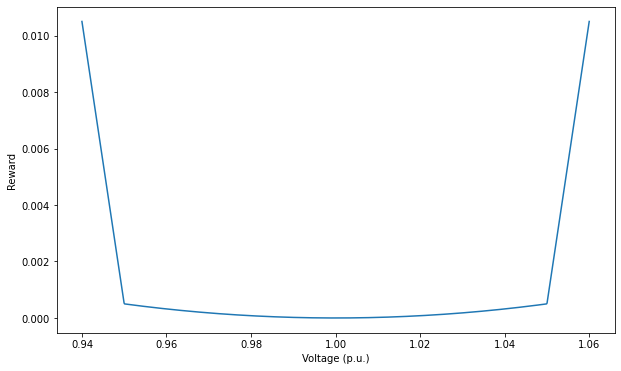
\includegraphics[width=.4\linewidth]{images/MVOberr/RL/volatge_violation_function.png}
            \caption[Voltage violation function]{Shape of the voltage violation function centred in 1 \gls{pu}}
        \end{figure}
        \noindent The idea is to punish the agent by a low value when the voltage bus is in the range [0.95,1.05] and to punish it more when the voltage bus is more far away from 1 \gls{pu}
        \[
            reward\_vv_t = -\sum_{i=0}^{|\mathcal{B}|} f(\mathcal{B}^{V}_{t+1,i})
        \]
        
        \item A reward for the critical situation solved. The agent is given a positive or negative reward whether it was able to solve the critical situation or not. In particular:\\
        \[
            reward\_cs_t =  C_{t+1} - 4 \cdot network\_status_{t+1}
        \]
        with $C_{t+1}$ the critical status of the network as stated in the forecasting section (expression \ref{eq:labels}) at time step $t+1$, and $network\_status_{t+1}$ a boolean value stating if the system at time step $t+1$, after the agent's action and the \gls{PF} calculation, is critical or not.\\
        The main idea is to make the agent understand if the chosen action was helpful and solved the critical situation of the network. In particular, there are four possible cases:\\
        
        \begin{itemize}[leftmargin=2cm]\label{im:cases}
            \item[case 1)] 0 - 0: no critical situation before and after the agent's action (good case, $0$ reward).
            \item[case 2)] 0 - 1: no critical situation before, but it was introduced by the agent's action (the worst case, $-4$ reward).
            \item[case 3)] 1 - 0: critical situation before and it was solved by the agent's action (the best case, $+1$ reward).
            \item[case 4)] 1 - 1: critical situation before and after the agent's action (not good case, $-3$ reward).
        \end{itemize}
        
        
        
    \end{itemize}
    The total reward is given by the algebraic sum of all the previous terms multiplied by a scaling factor:
    \begin{equation} \label{eq:rew}
      \begin{aligned}
            reward_t = &\hphantom{..,,} 
                          \alpha_p \cdot reward\_p_t + \\
                       &+ \alpha_q \cdot reward\_q_t + \\
                       &+ \beta \cdot reward\_vv_t + \\
                       &+ \gamma \cdot reward\_cs_t
      \end{aligned}
    \end{equation}
    with $\alpha_p=4$, $\alpha_q=2$, $\beta=100$ and $\gamma=20$. These values are chosen to balance the rewards get by the agent.\\
    With such articulate reward expressed in \ref{eq:rew}, the agent's goal is to reduce the number of over voltage situation without introducing new under voltage situations.
    
    \item \emph{Agent}. The agent model chosen is the \gls{DDPG} algorithm. As mentioned in \ref{sssec:ddpg}, this algorithm can handle continuous state and action spaces, so it is suitable for this task.\\
    
    Both actor and critic networks are \glspl{MLP} composed by three hidden layers with 256, 128, 128 neurons. The weights are initialised with a standard distribution with mean 0 and standard deviation $0.08$ so that most of the weights are concentrated between $[-0.1,0.1]$. This is important since with a larger initial standard deviation, the model tended to saturate the output.\\
    
    To control both the active and reactive power of the generators, the final hidden layer of the actor networks is sent to two different branches: one for $\mathbf{a^p}$ with a Sigmoid function as activation function, and the other branch for $\mathbf{a^q}$ with \gls{Tanh} as activation function and a scaling factor of $0.25$.
    
    Some other hyperparameters are:
    \begin{itemize}
        \item $\alpha$, the learning rate for the actor networks, set to $10^{-4}$.
        \item $\beta$, the learning rate for the critic networks, set to $10^{-3}$.
        \item $\tau$, the scaling factor for updating the weights with equation \ref{eq:polyak}, set to $10^{-3}$.
        \item The weights of the critic networks are updated every 3000 time steps.
        \item The agent is trained every 3 time steps.
        \item To the action is added some noise, initially set to 0.1, and it decreases every 100 time steps of a factor of 0.995. The noise minimum is set to $10^{-5}$, below this value the noise is not decreased any more.
        \item For all the networks, an Adam optimiser is used.
        \item The replay memory is set to $10^6$. After the memory is full, the past experiences are overwritten with the new ones.
    \end{itemize}
    
\end{itemize}

The agent is trained using $40\%$, $14016$ time steps, of the data and tested on the remaining $60\%$, $21024$ time steps. The training is repeated for $4$ time for a total of $56064$ time steps.\\

\begin{algorithm}[H]
  \caption{Pseudo-algorithm for the control of the network's devices}
  \begin{algorithmic}
    \STATE Initialise the network
    \STATE Extract time series for each time step from Simbench database
    \STATE Calculate \gls{PF} for each time step and evaluate when the system is in a critical situation, obtaining $\textbf{C}$
    \STATE Initialise agent with actor and critic networks: $\phi$, $\theta$, $\phi_{target}$ and $\theta_{target}$ 
    \FOR{ each episode $p$ } 
        \FOR{ each time step $t \in \{1,2,\dots,T-2,T-1\}$ }
            \STATE Get state $\mathbf{s_t}$ from the network
            \STATE Choose the action $\mathbf{a_t}$ with $\mathbf{a_t}=\phi(\mathbf{s_t})$
            \STATE Get active power of the generators at time step $t+1$: $\mathbf{initial\_power_{t+1}}$
            \STATE Apply the action $\mathbf{a_t}$: change active power with the $\mathbf{final\_power_{t+1}}$ and reactive power with $\mathbf{a^q_t}$ of the generators at time step $t+1$
            \STATE Calculate the \gls{PF} at the time step $t+1$
            \STATE Calculate the reward $r_t$, as mentioned in \ref{4:rewfunc}
            \STATE Check the status of the environment: $d_t$
            \STATE Get new state $\mathbf{s_{t+1}}$
            \STATE Store the experience ($\mathbf{s_t}, \mathbf{a_t}, r_t, \mathbf{s_{t+1}}, d_t$)
            \STATE Train the agent
        \ENDFOR
    \ENDFOR
  \end{algorithmic}
\end{algorithm}

It is worth mentioning that Pandapower allows performing time series analysis, but training the \gls{RL} agent required a custom control of the time series execution. For this reason, the open-source code of Pandapower is modified to allow a finer control of the different steps of the runs.\\
% Some hyperparameter used are:
% \begin{itemize}
%     \item the agent is trained every 2 time steps;
%     \item 
% \end{itemize}
